\chapter{Auto-encoding logic programs}\label{ch:alps}


This chapter discussed the third contribution of the thesis in the form of \textit{auto-encoding logic programs}.
Auto-encoding logic programs lift the auto-encoding principle from vector representation to logical data formats.
More precisely, it uses clauses logic for data representation and  as a computational framework for encoder and decoder functions.


The chapter is based on the following publications.

\begin{quote}
	\bibentry{Dumancic2018a}
\end{quote}

\begin{quote}
	\bibentry{AlpsSubmitted}
\end{quote}



\section{Introduction}




The previous chapter introduces \gls{curled} -- a method for relational representation learning that creates latent representation by exploiting symmetries in data.
Even though \gls{curled} brings concepts from the \gls{srl} into relational representation learning, it relies on the external clustering procedure to \textit{invent} new predicates.
Thus, the constructed representation hierarchy  is not truly relational as latent features are not defined through logical formulas, even though we managed to find a way to explain the meaning of the constructed features.
Additionally, latent representations created by \gls{curled} are prone to generating a rather large number of latent features, of which only a small portion  is actually used in the subsequent predictive model.
Though the discovered features are likely to be useful for many different tasks, they make the generative learning of \gls{srl} models difficult as a large number of predicates results in a large search space.





In this chapter we ask the following question: \textit{how can we learn latent representations of relational data in a principled framework that can keep data and reasoning at the relational level?}
We are interested in learning relational latent representation by means of learning and inference methods from the \gls{srl} community.



We argue that fully retaining first-order logic as a data representation language within deep learning approaches offers several benefits.
First, predicate logic is a Turing-equivalent programming language and thus provides a language that does not introduce any limitations upfront.
Second, it is easily interpretable (whereas \gls{dl} is a \textit{black-box}) and modular which might allow for efficient learning strategies.
Third, once the domain model is obtained, \gls{srl} systems can answer any question w.r.t. the provided domain model and the user thus does not have to commit to a specific learning task in advance.
Fourth, \gls{srl} and other logic-based ML methods are very data-efficient and capable of learning from a few examples only, whereas \gls{dl} is \textit{data-hungry}.
Fifth, SRL methods allow for incorporation of \textit{background knowledge} and thus can easily build further on previously gathered knowledge.






This work takes a fresh look at the representation learning problem and induces relational latent representations in a \textit{symbolic way}, instead of the gradient-based optimisation.
We introduce \textit{auto-encoding logic programs} (\alp{s}) -- a novel relational \gls{dl} component which uses logic programs as a computation engine instead of neural networks.
We focus on auto-encoders as they have proven to be among the most versatile \gls{dl} primitives and applicable to different learning settings (un-, semi- and supervised learning) using the same learning principle \cite{SSLVAE2014,VincentDaE,Kingma2014,BengioSAE}.
This versatility is important as it makes a single latent representation suitable for many tasks within \gls{srl}.
There tasks range from learning predictive models to structure learning.
A key difference between the predicate invention approaches and \alp{s} is that that we create latent representations in an entirely unsupervised manner, whereas predicate invention is defined as a supervised method.
An exception to that is the work related to \textit{statistical predicate invention}~\cite{Kok2007} which also addresses a generative learning setup within \gls{srl}, but never explicitly creates latent representation.
Moreover, it is not used to provide novel language constructs to an \gls{srl} learner, but only to compress the existing KB by identifying entities \textit{identical} to each other and thus speed up learning~\cite{Kok:2009:LML:1553374.1553440}.
If one would explicitly construct the latent representation, learning generative models would be extremely difficult due to the very large number of created constructs.
%\wannes{True for all methods? Eg Kok's SPI (they state ``The invented predicates capture arbitrary regularities over all relations, and are not just used to predict a designated target relation.'' + evaluate AUC)?}.
%\wannes{show what is now possible that wasn't before}




First learning a latent representation can be beneficial for the main learning task of \gls{srl}, namely structure learning, in which the goal is to find a set of formulas and the corresponding probabilities.
The main reason why (structure) learning in \gls{srl} is a difficult problem is that the learning task is in its core a search problem with the aim of identifying a small set of predictive logical formulas.
Therefore, it suffers from the combinatorial explosion which comes from a large number of logical formulas that can typically be constructed given a fixed vocabulary.
Interpreting candidate formulas as individual features, this is reminiscent of the problem of learning from high-dimensional spaces, which is the problem DL tackles.
Therefore, incorporating \gls{dl} ideas into \gls{srl} might reduce the complexity of structure learning and/or increase the quality of the obtained models.
%\tias{this paragraph brutally switches to the learning task, can use smoother transition. E.g: 'First learning a latent representation can be beneficial for the main learning task of SRL, namely structure learning. ...'}


The contributions of this work are a (i) \textit{a framework for learning auto-encoding logic programs} which is both data-driven and data-efficient, interpretable, and unsupervised, which means that the resulting latent representation is suitable for many \gls{srl} learning tasks; (ii) \textit{a generic procedure to cast learning the auto-encoders as a constraint optimisation problem, for which existing efficient solvers can be used}; and (iii) \textit{an experimental evaluation of the proposed framework that shows the benefits for generative learning}.





\section{Auto-encoding Logic Programs}

\begin{sidewaysfigure}
	\centering
    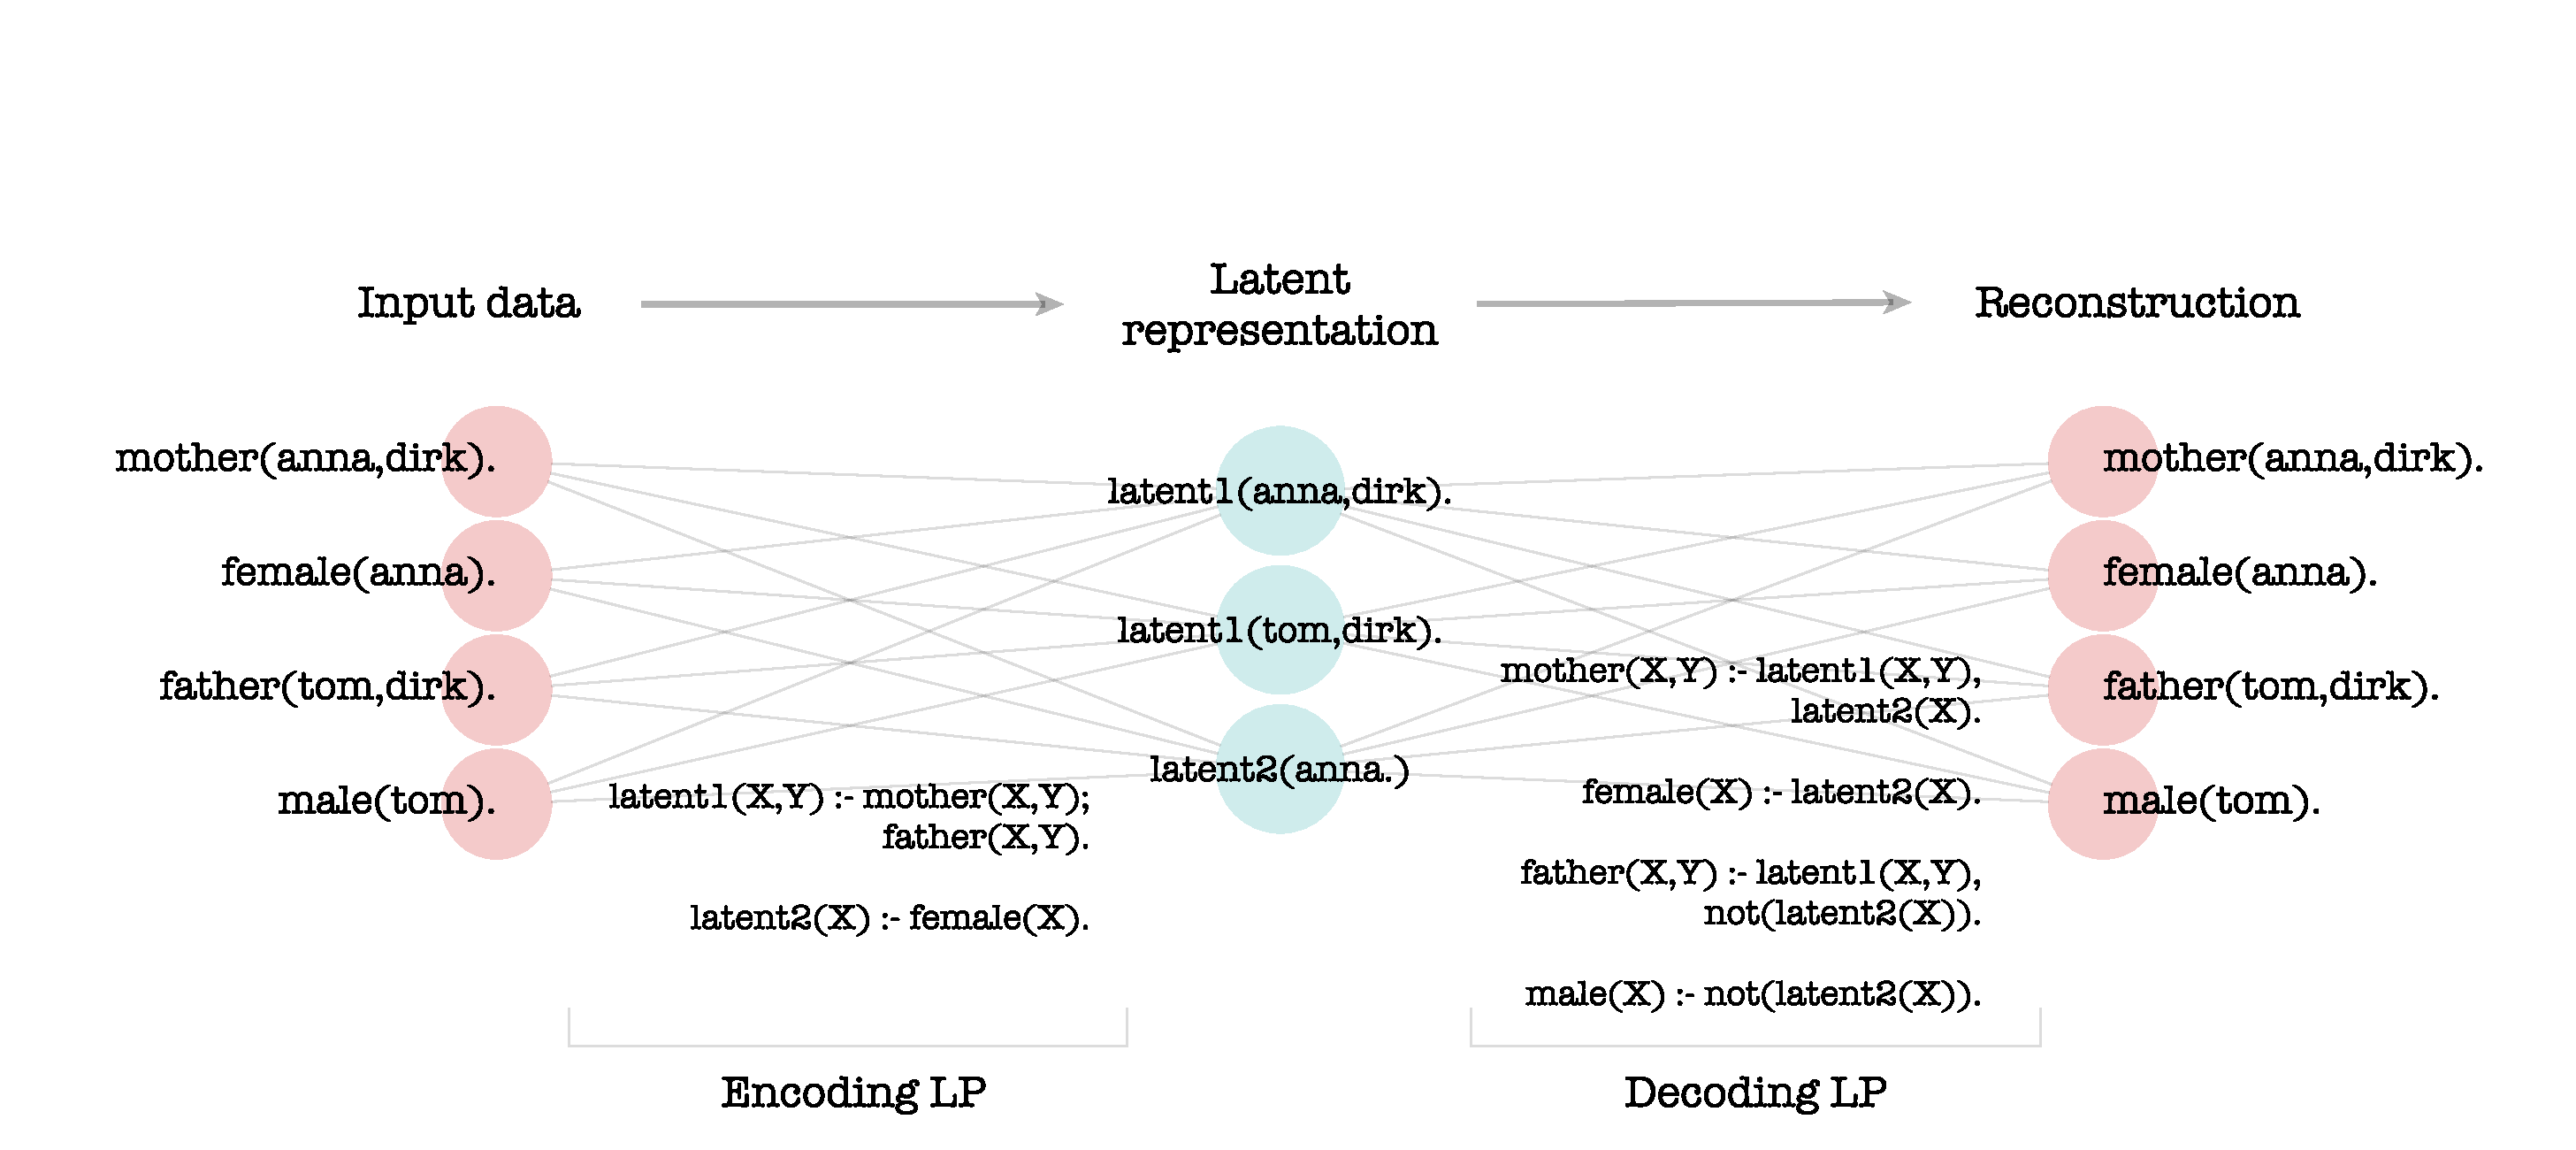
\includegraphics[width=.95\textwidth]{alps}
    \caption[Illustration of the Auto-encoding logic programs]{Illustration of the auto-encoding logic program learning the concept of \textit{parent} in the latent representation (underlay figure of neural auto-encoder for convenience).\label{fig:alp}}
\end{sidewaysfigure}



The core idea of auto-encoders is the \textit{reconstruction principle}: the goal is to learn an \textit{encoder}, mapping the provided data to its latent representation, and a \textit{decoder}, reconstructing the original data from the latent space, such that the reconstruction is maximal.
The key ingredient of their success is the limited capacity of the latent representation, ensured by limiting its dimensionality and enforcing sparsity.
\textit{Traditional} auto-encoders use vectors as a data representation format, and matrices to represent the mapping functions for encoder and decoder.


Intuitively, our goal is to lift the framework of auto-encoders to use \textit{first-order logic as a data representation language},  and \textit{logic programs} as mapping functions of the encoder and decoder (Figure \ref{fig:alp}).
It is important to note that by assimilating logic programs, the mapping functions of \alp{s} are realised in a Turing-complete language, giving them the potential to learn arbitrarily complex latent representations.




\paragraph{Preliminaries.}
In order to formalise the learning framework, let $\mathcal{KB}$ be a knowledge base (a set of facts) with a vocabulary $\mathcal{V} = \{ \mathcal{P}, \mathcal{C}\}$ where $\mathcal{P}$ is a set of predicates and $\mathcal{C}$ a set of constants.
Let $\mathcal{L}$ be a set of predicates not in $\mathcal{P}$; these predicates are called \textit{latent predicates}.
Let $\mathcal{KB}_{\mathcal{L}}$ be a \textit{latent knowledge base} with a vocabulary $\mathcal{V}_{\mathcal{L}} = \{\mathcal{L}, \mathcal{C}\}$.
Let $\mathcal{HB(P,C)}$ be a \textit{Herbrand base} - a set of all ground atoms composed with $\mathcal{P}$ and $\mathcal{C}$ (equivalently for $\mathcal{HB(L,C)}$).
Then $\mathcal{KB} \subset \mathcal{HB(P,C)}$ and $\mathcal{KB}_{\mathcal{L}} \subset \mathcal{HB(L,C)}$ with a constraint that $\forall e \in \mathcal{KB}, e = true$ (under the \textit{closed-world assumption}, everything not specified as \textit{true} is \textit{false}).



\paragraph{The framework.}
The individual components of the framework are defined as follows.



\begin{definition}
\textbf{Relational encoder.}
A \textit{relational encoder} (Figure \ref{fig:alp}, left) is a logic program $\mathcal{E}$ %$: \mathcal{HB(P,C)} \rightarrow \mathcal{HB(L,C)}$
that maps a set of facts $\mathcal{KB} \subset \mathcal{HB(P,C)}$ to a set of latent facts $\mathcal{KB}_{\mathcal{L}} \subset \mathcal{HB(L,C)}$.
The clauses of the encoder are termed \textit{encoder clauses} and their bodies consist of predicates in $\mathcal{P}$, while the heads are composed of predicates in $\mathcal{L}$.
\end{definition}


\begin{definition}
\textbf{Relational decoder.}
A \textit{relational decoder} (Figure \ref{fig:alp}, right) is a logic program $\mathcal{D}$ %$: \mathcal{HB(L,C)} \rightarrow \mathcal{HB(P,C)}$
that maps a set of latent facts $\mathcal{KB}_{\mathcal{L}} \subset \mathcal{HB(L,C)}$  to a new set of facts $\mathcal{KB}' \subset \mathcal{HB(P,C)}$.
The clauses are termed \textit{decoder clauses} and their bodies consist of predicates in $\mathcal{L}$, while the heads are predicates in $\mathcal{P}$.
\end{definition}



\begin{definition}
\textbf{Auto-encoding logic program (\alp{}).}
An \textit{auto-encoding logic program} is a logic program that, given a knowledge base $\mathcal{KB}$, constructs encoder $\mathcal{E}$ and decoder $\mathcal{D}$ programs, together with the latent predicate vocabulary $\mathcal{L}$.
\end{definition}


For defining the loss for the \alp{s}, we differentiate between \textit{true reconstructions} -- ground atom that are indicated as \textit{true} in the given knowledge base $\mathcal{KB}$, and \textit{false reconstruction} -- ground atoms produced by the decoder but not present in $\mathcal{KB}$.

\begin{definition}
\textbf{Knowledge base reconstruction loss.}
The knowledge base reconstruction loss (the difference of the leftmost and rightmost part of Figure \ref{fig:alp}), $loss(\mathcal{E}, \mathcal{D}, \mathcal{KB})$, is defined as

\begin{equation}
    loss(\mathcal{E},\mathcal{D},\mathcal{KB}) = | \mathcal{D}(\mathcal{E}(\mathcal{KB})) \, \ominus \, \mathcal{KB} |
    \label{eq:reconstruction}
\end{equation}


where $\ominus$ is the symmetric difference between two sets (the given knowledge base $\mathcal{KB}$ and the decoded $\mathcal{D}(\mathcal{E}(\mathcal{KB}))$), which returns (1) all non-reconstructed facts from $\mathcal{KB}$ and (2)  all \textit{false} reconstructions.
%\tias{changed 'a symmetric diff' to 'the symm diff' assuming there is only one? I prefer $\ominus$ btw as the diff is more explicit}
\end{definition}



In defining the task of learning relational auto-encoders we closely follow the learning task of \textit{inductive logic programming}, and make use of \textit{background knowledge} and \textit{language bias}.
Background knowledge represents additional knowledge about the domain a user might have, typically a set of rules, which is not present in the $\mathcal{KB}$ (for instance, a rule saying that every mother is a good cook \textit{good\_cook(X) :- mother(X,Y).}).
It can be used while constructing the encoder candidates, but is not part of the reconstruction.
A language bias is a set of instructions on how to syntactically compose candidate clauses (typically specified using syntactic constraints, e.g., all conjunctive and disjunctive formulas containing at most 3 literals and at most 2, existentially quantified, variables) (see Supplementary material for details).
%\tias{mention that allow disj too?}
This defines a set of \textit{candidate} encoder and decoder clauses.



\begin{definition}
\textbf{Learning \alp{s}.}
\textbf{Given} a (set of) knowledge base(s) and background knowledge about the domain, a language bias and constraints on the latent representation, \textbf{find} a set of encoder and decoder clauses that minimise Equation \ref{eq:reconstruction}.
\end{definition}

By constraints on latent representation we mean any constraint that affects the interactions of latent predicates; for example, stating that the latent $\mathcal{KB}$ can have at most $N$ facts.



\section{Learning as constraint optimisation}

In this section we show how the above defined problem of learning \alp{s} can be cast as a \textit{constraint optimisation problem} (COP) \cite{Rossi:2006:HCP:1207782} and provide a general principle how to map the learning problem to a set of constraints.
We chose COP as a target solver paradigm as it allows us (1) to deal with large search spaces (current COP technology can deal with millions of variables, which is the scale of DL problems and much larger than traditional logic programs) and (2) to specify the problem declaratively, that is, by describing the problem and including the objective function, but without providing the solving procedure.
%\tias{a pref? is very different, do you mean 'including the objective function'? Note that LNS does require some specification... Alt: and using one of the many built-in search procedures}


Intuitively, the mapping is done in the following way.
The language bias provided by the user determines all possible candidate encoder clauses. This is done by specifying all logical formulas that can be used as bodies as encoder clauses, and appending a fresh latent predicate as the head.
Having the candidate encoder clauses, all possible decoder clauses are specified in the same manner.
The problem now consists of selecting a subset of encoder and decoder clauses that satisfies all constraints and gives the minimal reconstruction loss.



A \textit{constraint optimisation problem} consists of three components: \textbf{decision variables} whose values have to be assigned, \textbf{constraints} on values and interaction of decision variables, and an \textbf{objective function} stating the preference over the assignments of values to decision variables. We build a COP to learn an \alp{}  as follows.


\paragraph{Decision variables.}
Each candidate encoder and decoder clause is associated with a \textit{Boolean decision variable} which indicates whether a clause is selected (having the value 1) or not (having the value 0).


\paragraph{Objective function.}
The objective function captures the reconstruction ability of a certain selection of encoder and decoder clauses by means of Equation \ref{eq:reconstruction}: $loss(\mathcal{E},\mathcal{D},\mathcal{KB}) = | \mathcal{D}(\mathcal{E}(\mathcal{KB})) \, \Delta \, \mathcal{KB} |$.
To compute this, we have to know which facts in $\mathcal{KB}$ each of the decoder clauses reconstructs, as well as which facts not present in $\mathcal{KB}$ are reconstructed.
This can be achieved by first executing the encoder, and using the obtained latent facts to execute the decoder.
%This further allow us to write the objective function in Equation \ref{eq:reconstruction} in terms of the decision variables, which we do  by means of \textit{soft constraints} that indicate the relationship between individual facts and decoder clauses that reconstruct them.
We can now create Boolean literals representing for all possible facts whether it is (re)constructed by a decoder clause or not.
%\tias{rewrote this sentence, please check that it matches what you mean because it was too loose}

For instance, assume that the fact \texttt{mother(anna,dirk)} can be reconstructed with any of the following two decoder clauses:
\begin{center}
	\texttt{mother(X,Y) :- latent1(X,Y),latent2(X).}

	 \texttt{mother(X,Y) :- latent3(X,Y).}
\end{center}

Assuming that the two clauses correspond to the decision variables \texttt{dc}$_1$ and \texttt{dc}$_2$, we add the constraint %turn this into a soft constraint \tias{this is not a soft constraint for me... though you will use it in the objective}.

\begin{center}
\texttt{rf}$_i \Leftrightarrow$  \texttt{dc}$_1  \vee $ \texttt{dc}$_2$
\end{center}

where \texttt{rf}$_i$ is a new Boolean variable propagating the information whether fact \texttt{mother(anna,dirk)} is reconstructed or not.
$\Leftrightarrow$ is the reification operator, ensuring that \texttt{rf}$_i$ is assigned to 1 if at least one of the decoder clauses \texttt{dc}$_1$ and \texttt{dc}$_2$ is selected.

%Using these \texttt{rf} variables, we can formulate the objective function by counting how many \textit{true} facts are not reconstructed and how many \textit{false} facts are introduced: %\tias{should probably use 'fact (not) present in KB' rather than true/false.}
Using these \texttt{rf} variables, we can formulate the objective function by counting how many facts present in $\mathcal{KB}$ are not reconstructed and how many atoms not present in $\mathcal{KB}$ are being reconstructed:
\begin{equation}
	\min \underbrace{\sum_{i=1}^{N}\text{not}(\text{\texttt{rf}}_i)}_{\text{\textit{true} reconstruction}} +  \underbrace{\sum_{j=1}^{M} \bar{\text{\texttt{rf}}_j}}_{\text{\textit{false} reconstruction}}
\end{equation}
where $N$ is the number of facts, and $M$ the number of false reconstructions (indicated with a bar, $\bar{\text{\texttt{rf}}}$). % \tias{hmm, wording can be clarified I think, e.g. 'present not present in kb' or smth. Also, does not need special 'bar' imho... (also note that bar sometimes means negation of the literal}
The optimisation task then corresponds to finding the assignment to decision variables that minimise the reconstruction loss.

%\tias{up to here, will continue later}


\paragraph{Constraints.}
Constraints have two primary functions in the proposed framework: (1) imposing the \textit{capacity constraint} which controls sparsity in the latent representation, and (2) imposing structure on the search space to speed up the search for the solution.


\textit{Capacity constraints}, such as sparsity or compression, are the key ingredient of \textit{traditional auto-encoders} preventing them from learning the \textit{identity mapping} as the latent representation.
We impose such a constraint by limiting the \textit{average number of facts per latent predicate} through the following hard constraint
$$ \frac{\sum_{i=1}^{N}w_i\text{\texttt{ec}}_i}{\sum_{i=1}^N\text{\texttt{ec}}_i} \leq \gamma G$$
where \texttt{ec}$_i$ are decision variables corresponding to the encoder clauses, $w_i$ indicates the number of latent facts they entail and which can be pre-computed, $\gamma$ is the \textit{compression parameter} and $G$ is the average number of facts in the original data representation.
We have also tried a more straightforward constraint of limiting the number of facts in the latent representation which gives worse results, so we do not consider it further.


The constraint problem specified so far is sufficient to find the latent representation, but search progresses very slowly.
To tackle this issue, we impose more structure in the search space by means of the following types of constraints.

\textit{Connecting encoder and decoder.}
A large part of the search space can be cut out by noticing that the encoder clauses deterministically depend on the decoder clauses.
This reduces the problem to searching only over decoder clauses, and retaining only the encoder clauses needed to construct selected decoder clauses.
To achieve this, we impose constraints of the following two types:
\begin{center}
	\texttt{dc}$_k$ $\Rightarrow$ \texttt{l$_i$ $\wedge$  l$_j$}

    \texttt{l}$_i$ $\Rightarrow$ \texttt{dc$_m$ $\vee$ dc$_n$}
\end{center}
The first constraint states the if a decoder clause \texttt{dc}$_k$ is selected, then encoder clauses \texttt{l$_i$} and \texttt{l$_j$} have to be selected as well (assume they are used in the body of \texttt{dc}$_k$).
The second constraint state that an encoder clause \texttt{l}$_i$ can be selected only if at least one of the decoder clauses using it in the body, \texttt{dc$_m$} and \texttt{dc$_n$}, is selected.


\textit{Refinement constraints.}
Given the limited capacity of the latent representation, it is desirable to encourage diversity among the selected latent predicates, and prevent the solver from exploring regions where encoder clauses are too similar (yielding marginal gain).
Assume that a clause \texttt{ec}$_1$ is a direct refinement of another clause \texttt{ec}$_2$, i.e., \texttt{ec}$_1$ is obtained by adding a literal to the body of \texttt{ec}$_2$.
As \texttt{ec}$_1$ introduces only a subset of atoms reconstructed by \texttt{ec}$_2$, we cannot gain anything by selecting both clauses.
Therefore, we introduce the following constraint

$$ !(\text{\texttt{ec}}_1 \wedge \text{\texttt{ec}}_2) == \text{\texttt{true}} $$
simply stating that both clauses can not be part of the solution together.



\textit{Syntactic variants.}
A common way to reduce the search space in relational learning is to remove \textit{syntactic variants}.
Two encoder clauses are syntactic variants if they have the same head predicate and entail the same facts.
Therefore, including a clause that is a syntactic variant of the clause already in the solution does not yield any benefit.
However, syntactic variants cannot be simply excluded from the search as some two syntactic variants might depend on different encoder clauses.
To ensure only one of the syntactic variants is part of the solution, we impose the following constraint, assuming that \texttt{dc}$_1$,\texttt{dc}$_2$, \texttt{dc}$_3$ are syntactic variants:

\begin{center}
	\texttt{dc}$_1$ + \texttt{dc}$_2$ + \texttt{dc}$_3$ $\leq$ \texttt{1}.
\end{center}




\textit{Reconstruct all predicates.}
%In order to prevent the solver from getting stuck in a local minimum that only reconstructs facts related to a subset of predicates, we introduce a constraint stating that for each predicate in $\mathcal{P}$, at least one decoder clause with that predicate as head has to be selected.\tias{too long sentence}
Assume that \texttt{dc}$_k$,\texttt{dc}$_l$ and \texttt{dc}$_m$ are decoder clauses all having predicate $p$ as the head predicate.
we introduce the following constraint to state that at least one of them has to be selected: %\tias{the ==1 is highly unconventional, just leave it out? or at least == true like you did earlier}
$$ \text{\texttt{dc}}_1 \vee \text{\texttt{dc}}_2 \vee \text{\texttt{dc}}_3 == \text{\texttt{true}}.$$
We have noticed that this constraint allows the solver to find good solution faster; the reason being that this constraint eliminates the solutions that reconstruct well one predicates with a high number of facts while ignoring other predicates with a lower number of facts.



\subsection{Search}

Given the combinatorial nature of \alp{s}, exact and complete search is impossible in all but the smallest problem instances.
Therefore, we resort to a standard technique in constraint programming, namely \textit{large neighbourhood search} (LNS) \cite{Ahuja:2002:SVL:772382.772385}. LNS combines complete search with random exploration.
It imposes a limit on the number of backtracks for individual runs of a complete search; once the limit is reached, it restarts the search in a random neighbourhood around the current best solution.
This is typically done by assigning a small portion of decision variables to their values in the best solution found so far, and searching over the remaining variables.


A key design choice in applying LNS is how to define the neighbourhood.
We introduce the following \textit{remember-forget} strategy for constructing neighbourhoods.
The strategy is based on noticing that the solution is necessarily sparse - only a tiny proportion of candidate decoder clauses will be a part of the solution at any time.
Therefore, when restarting it is important to preserve at least some of the selected decoder clauses from the best solution so far.
Assume $\mathcal{B}$ is the assignment of variables corresponding the best solution found so far.
Let a variable be \textit{active} if it is selected in $\mathcal{B}$, and \textit{inactive} otherwise.
We construct the neighbourhood by \textit{remembering} the value assignments of $\alpha$ \% active variables (corresponding to decoder clauses), and \textit{forgetting} (i.e., setting the value to 0) $\beta$ \% of candidate encoder clauses.
For the individual search runs, we use \textit{last conflict search} \cite{COS} and the \textit{max degree} ordering of decision variables.




\subsection{Pre-processing}
As the candidate clauses are generated purely syntactically, many of the candidate will be uninformative and introduce many false reconstructions.
We can further reduce the number of candidates, and hence the search space, through the following pre-processing steps that use specific properties of the problem at hand:


\begin{definition}
\textbf{Naming variants.}
Given two encoder clauses \textit{ec$_1$(X):\!-...}
%p1(X,Y),p2(Y)}
and \textit{ec$_2$(X):\!-...}
% p3(X,Y),p2(Y).}
with \textit{L1=\{ec$_1$(a),ec$_1$(b),...\}} and \textit{L2=\{ec$_2$(a),ec$_2$(b), ...\}} the respective sets of true instantiations.
The two clauses are \textit{naming variants} if renaming the predicate names in \textit{L1} and \textit{L2} to a common name yields identical sets \textit{L1} and \textit{L2}.
\end{definition}


In order to reduce the search space, we detect all naming variants and keep only one instance as a candidate.


\begin{definition}
\textbf{Signature variants.}
Assume two decoder clauses, \texttt{dc}$_m$ and \texttt{dc}$_n$, with the same head predicate.
Let \texttt{C}$_m$ (\texttt{C}$_n$) be the maximal set of facts decoder clauses \texttt{dc}$_m$ (\texttt{dc}$_n$) entail, and \texttt{B}$_m$ (\texttt{B}$_n$) be the maximal set of predicates used in the body of the two clauses.
The two clauses are \textit{signature variants} if \texttt{C}$_m$ $=$ \texttt{C}$_n$ and \texttt{B$_m$} $=$ \texttt{B$_n$}.
\end{definition}

As signature variants are redundant w.r.t. the optimisation problem, we keep only one of the clauses detected to be signature variants and remove the rest.


\begin{definition}
\textbf{Corruption level.}
Given a decoder clause \texttt{dc}$_i$, its true instantiations \texttt{DC} and the original interpretation $\mathcal{KB}$, the \textit{corruption level} is defined as $c(\text{\texttt{dc}}_i) = \frac{|e \in \texttt{DC}\ \wedge\ e \not \in \mathcal{KB}|}{|\text{\texttt{DC}}|}$.
\end{definition}

The notion of the \textit{corruption level} turns out to be particularly important, because if $c(\text{\texttt{dc}}_i) \geq 0.5$ then the decoder clause \texttt{dc}$_i$ cannot improve the objective function as it introduces more \textit{false positives} than \textit{true positives} (under the assumption that the false reconstructions are not shared between the decoder clauses).
We remove the candidate clauses that have a corruption level $\geq 0.5$.





\section{Experiments and results}



The experiments aim at answering the following question:

\begin{displayquote}
\textit{Does inducing a latent  representation with \alp{s} help with solving SRL tasks?}
\end{displayquote}

We focus on evaluation in a generative learning settings, and focus on learning generative \textit{Markov Logic Networks}~\cite{Richardson2006}.
This means, more precisely, that we are interested in whether learning the structure of a generative model in the \textit{latent space}, and decoding it back to the original space, is more effective (in terms of how well it explains the data) than learning the model in the original data space.


To answer the question, we apply the following procedure.
The baseline \gls{mln} model is simply learned on the original data representation, and the average \textit{leave-one-out} AUC-PR is reported.
We report AUC-PR instead of AUC-ROC because AUC-PR is less sensitive to the class imbalance problem~\cite{Davis:2006:RPR:1143844.1143874}, which is the case with the datasets we use in the experiments.
To learn the \textit{latent} MLN model, we first learn the latent representation with \alp{s} varying the length of clauses and the compression level, and learn an \gls{mln} on the resulting latent representation.
To evaluate the learned \gls{mln}s, we query each fact regarding one specific predicate given everything else as evidence.
This is repeated for each predicate in a test interpretation.
In case of latent \gls{mln}, predicate is removed before the rest of the data is encoded to the latent space.
To allow for comparing the latent \gls{mln} with the baseline model, once the structure is learned in the latent space we append the corresponding decoder from ALPs to the latent model (see Supplementary material).
This ensures that the baseline and latent \gls{mln}s operate in the same space.
The only difference when performing inference with latent \gls{mln} is that each latent predicate that could have been effected by removal of the test predicate (i.e., the test predicate is present in the body of the encoder clause defining the specific latent predicate) has to be declared \textit{open world}, otherwise MLNs will assume that all atoms not present in the database are \textit{false}.


 We limit the expressivity of \gls{mln} models to only formulas of length 3 with at most 3 variables (also known as a liftable class of \gls{mln}s).
 %the reasoning being that the benefit of the latent representation is easier to measure if the model being learned is simple and
This does not sacrifice the performance of \gls{mln}s, as shown in \cite{VanHaaren2016} which achieves the state-of-the-art structure learning results while imposing the same restrictions to \gls{mln}s.
We use BUSL \cite{mihalkova:icml07} as a generative \gls{mln} learner.




When learning latent representations, we vary the length of encoder and decoder clauses in $\{2,3\}$ and the compression level (the $\alpha$ parameter) in $\{0.3, 0.5, 0.7\}$.
This choice of parameters expresses a trade-off between long, complex rules and the search space size.
Also, this does not exclude learning longer rules since several layers of latent predicates/\alp{s} can be \textit{stacked}.
This is a useful property in an \gls{srl} setting.
Suppose a formula of length 6 is ideal.
Instead of searching in a huge space to find such a formula, the latent representation captures short formulas and stacks those to build the longer formula of size 6.




\textbf{Data}
We use standard SRL benchmark datasets to evaluate \alp{s}.
\textit{WebKB} contains a set of web pages scrapped from four US universities - Cornell and Universities of Texas, Washington and Wisconsin.
The data contains web pages, their mutual links and more semantic information about relationships between pages, such as whether the page belongs to a student or a faculty member and courses they teach (we omit the word information, as in \cite{mihalkova:icml07}).
\textit{Cora-ER} contains a set of papers, their authors, title and venues, together entity resolution information (i.e., titles, authors and venues that refer to the same entities but are spelled differently).
\textit{UWCSE} contains the information about the employees of five departments at the CS department of University of Washington: student and professors together with mentorship relationships, courses they teach and so on.
We have experimented with other common SRL datasets, but have removed the on which BUSL did not manage to learn a model (AUC-PR $< 0.2$) (and IMDB on which no improvement was observed as the dataset is very easy to model).








\subsection{Results}



\begin{figure}
	\centering
    \begin{minipage}[thb]{.32\linewidth}
        \centering
        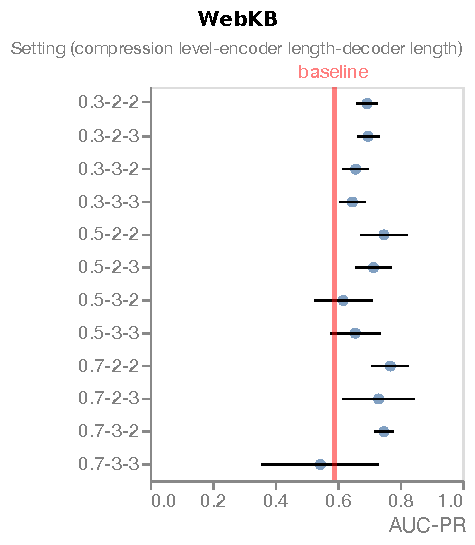
\includegraphics[width=.98\linewidth]{webkb_AUCPR_final}
    \end{minipage}
    \begin{minipage}[htb]{.32\linewidth}
        \centering
        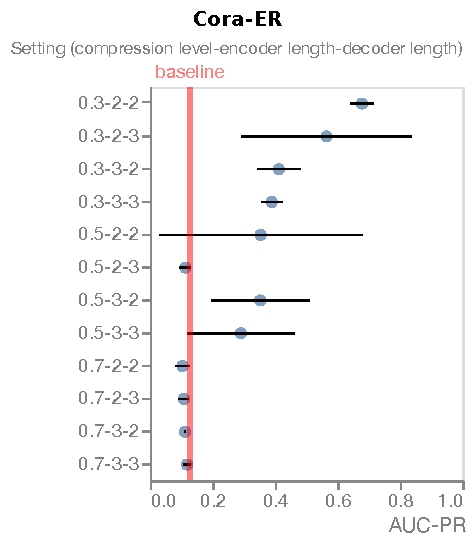
\includegraphics[width=.98\linewidth]{cora_AUCPR_final}
    \end{minipage}
    \begin{minipage}[htb]{.32\linewidth}
        \centering
        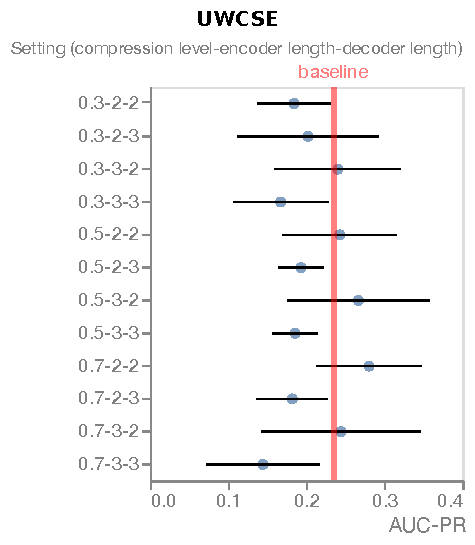
\includegraphics[width=.98\linewidth]{uwcse_AUCPR_final}
    \end{minipage}
    \caption[Performance of the \gls{mln} models learned on the original and \alp{s}-induced data representations.]{The \gls{mln} models learned on the latent representation outperform the baseline MLN (indicated with the vertical red line) in terms of the AUC-PR score, except on the UWCSE dataset where the gain is marginal.}
    \label{fig:resultsAUCPR}
\end{figure}





Figure \ref{fig:resultsAUCPR} summarises the performance, in terms of AUC-PR scores, of \gls{mln}s learned on the original data representation and various representation created by \alp{s} by modifying the clause lengths for both encoder and decoder, and varying the compression level of the latent representations.



%\begin{figure}
%	\centering
%	\includegraphics[width=.7\linewidth]{images/LossVsAUCPR_joint}
%	\label{fig:lossvsaucpr}
%	\caption{Relationship between reconstruction loss and AUC-PR scores. Color indicates datasets: Blue - Cora-ER;} Red - WebKB; Orange: UWCSE
%\end{figure}

The results indicate that latent representation created by \alp{s} are useful tool for relational learning.
The improvements are substantial for the WebKB and Cora-ER dataset: on the WebKB dataset the performance improves from $\approx 0.6$ to $\approx 0.8$, while on the Cora-ER dataset the score improves from $\approx 0.2$ to $\approx 0.7$.
However, the improvement on the UWCSE dataset if marginal -- it improves from $0.23$ to $0.28$.



The results also indicate that the quality of the latent representation depends highly on the chosen hyper-parameters, a property that is observed with the vast majority of representation learning approaches.
Whereas on WebKB all setups but one ($0.7-3-3$) improve the performance, the Cora-ER and UWCSE tend to be sensitive to the chosen parameters.
On Cora-ER, it seems to be important to compress the data heavily as setups with the compression level of $0.3$ perform the best.
One possible explanation is that Cora-ER contains a lot of word information; to find useful latent information about words, \alp{s} have to be forced to compress a lot, otherwise they are simply extracting patterns that are too general.

The results for the UWCSE dataset show that the performance gain is marginal, improved by only $0.05$ points, and most of the latent \gls{mln}s perform \textit{worse} than the baseline \gls{mln}s.
Upon further investigation, we discovered that marginal improvement is the result of \alp{s} getting stuck in local optima: this dataset has relatively large number of predicates  and therefore yielding a very large search space (Figure \ref{fig:timings}) which contains many local optima.
We noticed that these local optima had a particular \textit{cheat}: the encoder was composed of \textit{identity mappings} between the observed and the latent predicates and many specific encoder clauses that entail very small number of latent facts, resulting in having a small \textit{average number of facts per latent predicate} and cheating the capacity constraint.
We tried to circumvent this problem by imposing the constraint that prevent two decoder clauses, where facts entailed by one clause are a subset of facts entailed by the other clause, being selected together; however, that was computationally infeasible given the large number of candidate clauses.
Some results show that certain setups lead to the perfect reconstruction loss (Figure \ref{fig:lossvsaucpr}) -- this is the result of over-fitting.




\begin{figure}[t!]
	\centering
	\begin{subfigure}[t]{0.48\linewidth}
		\centering
		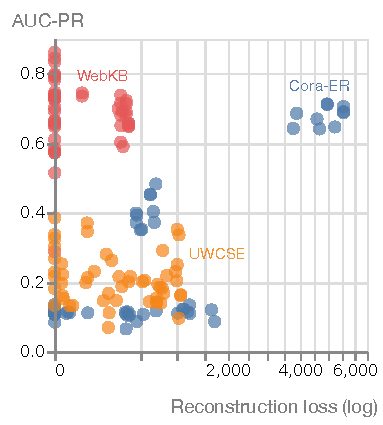
\includegraphics[width=.8\linewidth]{lossVsAUC}
		\caption{Relationship between reconstruction loss and AUC-PR scores. \label{fig:lossvsaucpr}}
	\end{subfigure}
	\hspace{.2em}
	\begin{subfigure}[t]{0.48\linewidth}
		\centering
		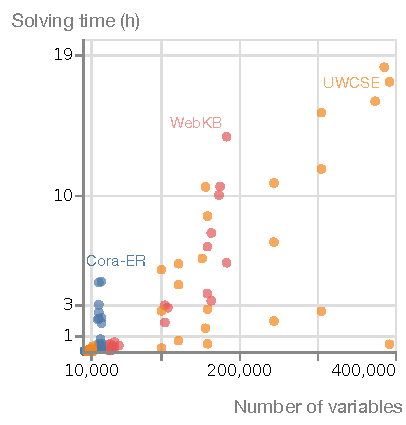
\includegraphics[width=.85\linewidth]{timings}

		\caption{Relationship between runtimes and the number of variables.\label{fig:timings}}
	\end{subfigure}
	\caption{Aspects of learning procedure for \alp{s}}
\end{figure}



It is interesting to see that there is no general trend relating reconstruction loss and performance (Figure \ref{fig:lossvsaucpr}).
On the WebKB, the best performing models are those with (near) perfect reconstruction; on the Cora-ER, the best performing models seems to have relatively high reconstruction loss; while on the UWCSE, the best performing models seem to occupy both parts of the spectrum.
This might indicate the amount of noise present in the data, suggesting that WebKB is a rather clean dataset, while Cora-ER contains quite some noise and the best performing models are learned on latent representation that manage to reduce the amount of noise.


Figure \ref{fig:timings} summarises the time needed for learning a  latent representation.
These timings show that, despite being defined as a combinatorial problem, \alp{s} are quite efficient: the majority of latent representations is learned within one hour, and a very few taking more than 10 hours (this excludes the time needed for setting the COP problem, as we did not optimise that step).
Moreover, the best result on each dataset (Figure \ref{fig:resultsAUCPR}) is rarely achieved with the latent representation with the most expressive \alp{} (with decoder clause length of 3, and any length of encoder clauses), which are the runs that take the longest.
This suggest that the length of clauses serves as a form of regularisation, and one can safely stick to the shorter clauses (and stacking if the complexity is needed) which are fast to learn.









\section{Conclusion}


We introduce \textit{Auto-encoding Logic Programs} (\alp{s}) -- a novel representation learning framework for representation learning with relational data.
The novelty of the proposed framework is that it learns a latent representation in a symbolic, instead of gradient-based way.
It achieves that by relying on first-order logic as a data representation language, which has a benefit of exactly representing the rich relational data without the need to approximate it in the embeddings spaces like many of the related works.
We further show that learning \alp{s} can be cast as a constraint optimisation problem, which can be solved efficiently in many cases.
We experimentally evaluate our approach and show that learning from the relational latent representations created by \alp{s} results in improved AUC-PR scores compared to learning in the original data representation.


%%%%%%%%%%%%%%%%%%%%%%%%%%%%%%%%%%%%%%%%%%%%%%%%%%
% Keep the following \cleardoublepage at the end of this file,
% otherwise \includeonly includes empty pages.
\cleardoublepage

% vim: tw=70 nocindent expandtab foldmethod=marker foldmarker={{{}{,}{}}}
